% =====================================================================
%  ASEAN Data Science Explorers 2026 — Storyboard
%  "Four Months' Notice"
%
%  Kompilasi:  pdflatex storyboard.tex   (jalankan 2x)
%  atau:       ./bangun.sh
%
%  Mesin sengaja pdflatex, bukan lualatex/xelatex: paket texlive-xetex dan
%  texlive-luatex belum terpasang di mesin ini, jadi fontspec + Noto Sans
%  tidak bisa dipakai. Font yang dipakai TeX Gyre Heros (klon Helvetica,
%  ikut texlive-fontsrecommended). Kalau nanti ingin Noto Sans:
%      sudo pacman -S texlive-xetex texlive-luatex
%  lalu ganti blok font di bawah dengan fontspec + \setmainfont{Noto Sans}.
%
%  ATURAN YANG DIPATUHI BERKAS INI
%   - PDF landscape 16:9 (960 x 540 bp), maks. 20 MB
%   - 15 halaman isi (batas resmi, sudah termasuk sampul); halaman Referensi
%     DI LUAR hitungan itu
%   - Sampul memuat 6 unsur wajib: judul, nama tim, institusi, negara,
%     SDG, deskripsi singkat
%   - SEMUA grafik wajib hasil SAP Analytics Cloud. Berkas ini hanya
%     menyediakan SLOT. Ekspor PNG dari SAC, taruh di gambar-sac/ dengan
%     nama persis seperti tertera di kotak placeholder, lalu kompilasi ulang
%     — slot otomatis berganti jadi gambar.
%   - Tiap gambar maks. 2 MB. Ekspor SAC minimal 1600 px lebar.
% =====================================================================

\documentclass[11pt]{article}

\usepackage[T1]{fontenc}
\usepackage[utf8]{inputenc}
\usepackage{textcomp}

\usepackage{geometry}
\geometry{paperwidth=960bp, paperheight=540bp,
          left=0bp, right=0bp, top=0bp, bottom=0bp,
          headheight=0bp, headsep=0bp, footskip=0bp,
          marginparwidth=0bp, marginparsep=0bp}

\usepackage{tgheros}
\renewcommand{\familydefault}{\sfdefault}
\usepackage{microtype}

\usepackage{tikz}
\usepackage{array}
\usepackage{colortbl}
\usetikzlibrary{calc}

\pagestyle{empty}
\setlength{\parindent}{0bp}
\setlength{\parskip}{0bp}
\setlength{\topskip}{0bp}
\setlength{\lineskip}{0bp}
\raggedbottom

% ---------------------------------------------------------------- data tim
\newcommand{\NamaTim}{Swallowgank}
\newcommand{\Institusi}{Institut Teknologi Sepuluh Nopember}
\newcommand{\Negara}{Indonesia}

% Nama produk di halaman 15. Ganti di sini saja kalau tim memilih nama lain.
% "Pawang" = kata Indonesia/Melayu untuk orang yang mengaku bisa membaca cuaca
% berbulan-bulan di muka. Namanya kelakar; isinya justru kebalikannya —
% aturannya terbuka dan bisa diperiksa tangan. Itu argumen dek ini.
\newcommand{\Produk}{Pawang}

% ---------------------------------------------------------------- palet
% Palet naskah: biru kasus, oranye alarm, merah puncak, abu konteks
\definecolor{accent}{HTML}{2A78D6}
\definecolor{alarm}{HTML}{E8833A}
\definecolor{peak}{HTML}{C53232}
\definecolor{muted}{HTML}{8A8F98}
\definecolor{ink}{HTML}{14202E}
\definecolor{soft}{HTML}{F2F5F9}
\definecolor{line}{HTML}{C9D3E0}
\definecolor{deep}{HTML}{0E2340}

% ---------------------------------------------------------------- tipografi
\newcommand{\navfont}{\fontsize{9}{11}\selectfont}
\newcommand{\eyefont}{\fontsize{10}{12}\selectfont\bfseries}
\newcommand{\headfont}{\fontsize{25}{29}\selectfont\bfseries}
\newcommand{\subfont}{\fontsize{15.5}{20}\selectfont}
\newcommand{\bodyfont}{\fontsize{13.5}{18.5}\selectfont}
\newcommand{\smlfont}{\fontsize{10.5}{14}\selectfont}
\newcommand{\tnyfont}{\fontsize{8.5}{11}\selectfont}
\newcommand{\kpifont}{\fontsize{44}{48}\selectfont\bfseries}
\newcommand{\kpimid}{\fontsize{30}{34}\selectfont\bfseries}

% ---------------------------------------------------------------- geometri
\newcommand{\PW}{960}
\newcommand{\PH}{540}
\newcommand{\ML}{36}
\newcommand{\MR}{924}
\newcommand{\CW}{888}
\newcommand{\CTOP}{424}   % batas atas area isi
\newcommand{\CBOT}{58}    % batas bawah area isi

% kanvas satu halaman
\newenvironment{halaman}{%
  \noindent\begin{tikzpicture}[x=1bp,y=1bp,inner sep=0bp,outer sep=0bp]
  \useasboundingbox (0,0) rectangle (\PW,\PH);
}{%
  \end{tikzpicture}\clearpage
}

% ---------------------------------------------------------------- daftar butir
\newenvironment{blist}{%
  \begin{list}{\raisebox{0.22em}{\textcolor{accent}{\rule{0.40em}{0.40em}}}}{%
    \setlength\leftmargin{1.15em}\setlength\labelwidth{0.7em}%
    \setlength\labelsep{0.45em}\setlength\itemindent{0bp}%
    \setlength\rightmargin{0bp}\setlength\topsep{0bp}%
    \setlength\partopsep{0bp}\setlength\parsep{0bp}\setlength\itemsep{8bp}}%
}{\end{list}}

% ---------------------------------------------------------------- komponen
% breadcrumb: \navbar{indeks aktif 1..8}, 0 = tanpa sorotan
\newcommand{\navbar}[1]{%
  \def\actv{#1}%
  \draw[line, line width=0.6bp] (\ML,506) -- (\MR,506);
  \foreach \i/\lbl in {1/{Problem},2/{Method},3/{Analysis},4/{Synthesis},%
                       5/{Solution},6/{Viability},7/{Impact},8/{Limits}}{%
    \pgfmathsetmacro{\cx}{36+111*(\i-0.5)}%
    \ifnum\i=\actv\relax
      \node[anchor=center, text=accent, font=\navfont\bfseries] at (\cx,517) {\lbl};
      \draw[accent, line width=2.2bp] ({\cx-32},506) -- ({\cx+32},506);
    \else
      \node[anchor=center, text=muted, font=\navfont] at (\cx,517) {\lbl};
    \fi
  }%
}

% kepala halaman: \kepala{eyebrow}{headline}
\newcommand{\kepala}[2]{%
  \node[anchor=north west, text=alarm, font=\eyefont] at (\ML,488) {\MakeUppercase{#1}};
  \node[anchor=north west, text width=\CW bp, align=left, text=ink, font=\headfont]
       at (\ML,472) {#2};
}

% kaki halaman: \kaki{sumber}{nomor}
% teks kaki di-anchor ke SOUTH west supaya kaki dua-tiga baris tumbuh ke ATAS,
% bukan meluber keluar halaman
\newcommand{\kaki}[2]{%
  \draw[line, line width=0.6bp] (\ML,50) -- (\MR,50);
  \node[anchor=south west, text width=780bp, align=left, text=muted, font=\tnyfont]
       at (\ML,12) {#1};
  \node[anchor=south east, text=muted, font=\tnyfont\bfseries] at (\MR,12) {#2};
}

% blok teks bebas: \teks{x}{y}{lebar}{isi}
\newcommand{\teks}[4]{%
  \node[anchor=north west, text width=#3bp, align=left, text=ink] at (#1,#2) {#4};
}

% kartu KPI: \kpi{x}{y}{lebar}{tinggi}{angka}{label}{warna}
\newcommand{\kpi}[7]{%
  \draw[rounded corners=4bp, fill=#7, draw=none] (#1,#2) rectangle ++(#3,-#4);
  \pgfmathsetmacro{\tw}{#3-28}%
  \node[anchor=north west, text width=\tw bp, align=left, text=white, font=\kpifont]
       at ({#1+14},{#2-10}) {#5};
  \node[anchor=south west, text width=\tw bp, align=left, text=white, font=\smlfont]
       at ({#1+14},{#2-#4+12}) {#6};
}

% -------------------------------------------------- SLOT GRAFIK SAC
% \sacslot{x}{y}{lebar}{tinggi}{nama-berkas}{judul grafik}{jenis + dataset}{resep}
% Kalau gambar-sac/<nama-berkas>.png ada  -> gambar dipasang.
% Kalau belum ada                          -> kotak placeholder berisi resep SAC.
% Judul dipasang sebagai node bernama; kotak digantung dari anchor south-west-nya,
% jadi judul satu baris maupun dua baris sama-sama tidak pernah menabrak kotak.
% (Catatan: \sbox/\settoheight TIDAK bisa dipakai di dalam tikzpicture.)
\newcommand{\sacslot}[8]{%
  \node[anchor=north west, text width=#3bp, align=left, text=ink,
        font=\smlfont\bfseries] (cap#5) at (#1,#2) {#6};
  \coordinate (tl#5) at ($(cap#5.south west)+(0,-5)$);
  \pgfmathsetmacro{\tw}{#3-32}%
  \IfFileExists{gambar-sac/#5.png}{%
    \node[anchor=north west] at (tl#5)
      {\includegraphics[width=#3bp,height=#4bp,keepaspectratio]{gambar-sac/#5}};
  }{%
    \draw[rounded corners=4bp, fill=soft, draw=line, dashed, line width=0.9bp]
         (tl#5) rectangle ++(#3,-#4);
    \node[anchor=north west, fill=accent, text=white, rounded corners=2bp,
          inner xsep=5bp, inner ysep=3bp, font=\tnyfont\bfseries]
         at ($(tl#5)+(10,-10)$) {SAC};
    \node[anchor=north west, text width=\tw bp, align=left, text=ink, font=\tnyfont]
         at ($(tl#5)+(10,-34)$) {\textbf{#7}\\[4bp]\textcolor{muted}{#8}};
    \node[anchor=south east, text=muted, font=\tnyfont]
         at ($(tl#5)+({#3-10},{-#4+8})$) {\texttt{gambar-sac/#5.png}};
  }%
}

% chip SDG
\newcommand{\sdgchip}[2]{%
  \tikz[baseline=(n.base)]{\node(n)[fill=#1, text=white, rounded corners=3bp,
    inner xsep=8bp, inner ysep=4bp, font=\smlfont\bfseries]{#2};}}

% ---------------------------------------------------------------- helper tabel
\newcommand{\thd}[1]{\textcolor{muted}{\tnyfont\bfseries\MakeUppercase{#1}}}

\begin{document}

% =====================================================================
% HALAMAN 1 — SAMPUL
% Enam unsur wajib panitia: judul, tim, institusi, negara, SDG, deskripsi
% =====================================================================
\begin{halaman}
  \fill[deep] (0,0) rectangle (\PW,\PH);
  % tiga pita palet cerita di tepi kanan: biru kasus, oranye alarm, merah puncak
  \fill[accent] (852,0) rectangle (888,\PH);
  \fill[alarm]  (888,0) rectangle (924,\PH);
  \fill[peak]   (924,0) rectangle (\PW,\PH);
  % blok bayangan halus supaya sisi kanan tidak kosong
  \fill[accent, opacity=0.10] (620,0) rectangle (852,\PH);

  \node[anchor=north west, text=alarm, font=\eyefont] at (60,478)
    {ASEAN DATA SCIENCE EXPLORERS 2026};

  \node[anchor=north west, text width=740bp, align=left, text=white,
        font=\fontsize{54}{58}\selectfont\bfseries] at (60,450)
    {Four Months' Notice};

  \node[anchor=north west, text width=700bp, align=left, text=white,
        font=\fontsize{21}{27}\selectfont] at (60,380)
    {Turning El Ni\~no into a dengue early-warning alarm for ASEAN};

  \draw[alarm, line width=3bp] (60,340) -- (160,340);

  \node[anchor=north west, text width=640bp, align=left, text=white,
        font=\subfont] at (60,320)
    {A freely available climate index gives ASEAN health offices months of
     warning before a dengue season turns severe. We turn that lag into a
     two-condition alert rule that any provincial health office can run today,
     with no model, no code and no paid data.};

  \node[anchor=north west, font=\smlfont] at (60,222)
    {\sdgchip{peak}{SDG 3 Health}\hspace{6bp}\sdgchip{accent}{SDG 13 Climate}\hspace{6bp}\sdgchip{alarm}{SDG 6 Water}};

  \draw[white, opacity=0.30, line width=0.6bp] (60,168) -- (800,168);

  \node[anchor=north west, text width=700bp, align=left, text=white,
        font=\bodyfont] at (60,148)
    {\textbf{Team \NamaTim} \quad\textcolor{line}{|}\quad \Institusi
     \quad\textcolor{line}{|}\quad \Negara};

  \node[anchor=south west, text=line, font=\smlfont] at (60,40)
    {All charts built in SAP Analytics Cloud \ $\cdot$ \ 100\% open data};
\end{halaman}

% =====================================================================
% HALAMAN 2 — THE PROBLEM (bobot 10%)
% =====================================================================
\begin{halaman}
  \navbar{1}
  \kepala{The problem}{Dengue is ASEAN's fastest-moving climate-sensitive disease}

  \kpi{36}{\CTOP}{300}{104}{1.26M}{cases in 2019, the worst year in our nine-country panel}{peak}

  \teks{36}{300}{300}{\bodyfont
    \begin{blist}
      \item Vietnam 368k $\cdot$ Philippines 220k $\cdot$ Thailand 159k
            \textcolor{muted}{(latest complete year per country)}
      \item The 2023--24 El Ni\~no added an estimated \textbf{9.6 million cases
            worldwide} \textcolor{muted}{(Tian et al., 2025)}
      \item Outbreaks are still fought \textbf{reactively}, only once cases surge
    \end{blist}}

  \sacslot{366}{\CTOP}{270}{348}{h02-tren-tahunan}{ASEAN dengue cases, 2000--2024}
    {Line chart --- \textit{Dengue national annual}}
    {Filter \texttt{complete}=True, \texttt{year} 2000--2024 $\cdot$
     Measure \texttt{cases} (Sum) $\cdot$ Dim X \texttt{year} $\cdot$
     Reference line di 2019, label ``record in our data''}

  \sacslot{654}{\CTOP}{270}{348}{h02-per-negara}{Cases by country, latest complete year}
    {Bar chart horizontal --- \textit{Dengue national annual}}
    {Measure \texttt{cases} $\cdot$ Dim \texttt{country} $\cdot$
     filter tahun lengkap terbaru (2022--2023) $\cdot$ urut menurun,
     biru; Indonesia disorot oranye}

  \kaki{Source: OpenDengue V1.3, national totals, complete-reporting years only.
        We do not claim a 2023--24 record, because our panel is incomplete for
        Vietnam and the Philippines after 2022.}{2}
\end{halaman}

% =====================================================================
% HALAMAN 3 — THE QUESTION
% =====================================================================
\begin{halaman}
  \navbar{1}
  \kepala{The question}{Climate data arrives months before patients do}

  \draw[rounded corners=4bp, fill=soft, draw=none] (36,\CTOP) rectangle ++(888,-86);
  \draw[alarm, line width=4bp] (36,\CTOP) -- (36,338);
  \node[anchor=north west, text width=852bp, align=left, text=ink,
        font=\fontsize{20}{26}\selectfont\bfseries] at (54,404)
    {Can a freely available climate index tell a health office how bad the coming
     season will be, early enough to act?};

  \teks{36}{306}{300}{\smlfont
    \begin{blist}
      \item \textbf{SDG target 3.3}: end the epidemics of neglected tropical
            diseases, of which dengue is one
      \item \textbf{SDG target 13.1}: strengthen resilience and adaptive
            capacity to climate-related hazards
      \item \textbf{SDG target 6.1}: safe water for all. Where piped water is
            absent, households store it, and \textit{Aedes} breeds in the store
    \end{blist}
    \vspace{9bp}
    \textbf{ASEAN priority.} Dengue sits under \textbf{ASEAN Health Cluster 2},
    \emph{Responding to All Hazards and Emerging Threats}, whose ASEAN Dengue Day
    statements ask member states for earlier and better coordinated action.
    \par\vspace{9bp}
    \textcolor{muted}{Our test: does the signal survive when we remove the seasonal
    cycle, hold out unseen years, and use the WHO outbreak definition?}}

  \sacslot{366}{306}{558}{232}{h03-alur}{From public index to public action}
    {Diagram --- SAC \textit{Shapes} + \textit{Text} (tanpa dataset)}
    {Empat kotak berurutan, panah di antaranya:
     \textbf{Climate index (ONI, monthly, public)} $\rightarrow$
     \textbf{3--4 month lag} $\rightarrow$
     \textbf{Dengue surge} $\rightarrow$
     \textbf{Action window: PSN/3M, larviciding, stockpiles}.
     Warna kotak mengikuti palet cerita: biru, abu, merah, oranye.}

  \kaki{The three tests promised here are answered on pages 7, 12 and 14.}{3}
\end{halaman}

% =====================================================================
% HALAMAN 4 — DATA & METHOD
% =====================================================================
\begin{halaman}
  \navbar{2}
  \kepala{Data \& method}{Nine open datasets, one monthly panel, zero paid sources}

  \node[anchor=north west] at (36,\CTOP) {%
    \begin{minipage}{564bp}
      \bodyfont
      \setlength{\arrayrulewidth}{0.5bp}
      \arrayrulecolor{line}
      \renewcommand{\arraystretch}{1.72}
      \begin{tabular}{@{}p{296bp}@{}>{\raggedleft}p{74bp}@{\hspace{18bp}}>{\raggedright\arraybackslash}p{176bp}@{}}
        \thd{Data} & \thd{Rows} & \thd{Coverage}\\[-2bp]
        \hline
        Dengue cases (OpenDengue V1.3)        & 70,397 & 10 countries, 1955--2025\\
        Dengue $\times$ climate monthly panel & 55,329 & province-month, lags pre-computed\\
        Temperature \& rainfall (CCKP, ERA5)  & 9,000  & monthly, 1950--2024\\
        ONI El Ni\~no index (NOAA CPC)        & 918    & monthly, 1950--2026\\
        Water \& sanitation (WHO/UNICEF JMP)  & 8,692  & 2000--2024\\
        Population (BPS Indonesia)            & 140    & provinces, denominators\\
        Flood exposure (GHSL)                 & 30,348 & 836 cities, 1975--2030\\
        \hline
      \end{tabular}
    \end{minipage}};

  \node[anchor=north west, font=\smlfont] at (36,146)
    {\sdgchip{peak}{SDG 3}\hspace{6bp}\sdgchip{accent}{SDG 13}\hspace{6bp}\sdgchip{alarm}{SDG 6}};

  \teks{36}{104}{564}{\smlfont
    \textcolor{muted}{Every table joins on the same two keys, \texttt{iso3} and
    \texttt{year}, with \texttt{period} added for the monthly
    dengue\,$\times$\,climate panel. Nothing is entered by hand.}}

  \draw[rounded corners=4bp, fill=soft, draw=none] (624,\CTOP) rectangle ++(300,-366);
  \node[anchor=north west, text=alarm, font=\eyefont] at (644,404) {METHOD};
  \teks{644}{382}{260}{\smlfont
    \begin{blist}
      \item Monthly national series, 2010+
      \item Lagged correlations, 0--4 months
      \item \textbf{Anomalies}: the seasonal cycle is removed before we accept
            any correlation
      \item A two-condition trigger rule
      \item Out-of-sample test on unseen years
      \item WHO/PAHO endemic-channel benchmark
    \end{blist}}

  \draw[line, line width=0.6bp] (644,124) -- (904,124);
  \node[anchor=north west, text width=260bp, align=left, text=accent,
        font=\smlfont\bfseries] at (644,110)
    {All charts built in SAP Analytics Cloud.};

  \kaki{Nine sources, all public: OpenDengue $\cdot$ World Bank CCKP (ERA5)
        $\cdot$ NOAA CPC $\cdot$ WHO/UNICEF JMP $\cdot$ BPS $\cdot$ GHSL
        $\cdot$ SIPSN KLHK $\cdot$ BNPB. No licence, no login, no cost.}{4}
\end{halaman}

% =====================================================================
% HALAMAN 5 — ANALYSIS 1: THE SEASON
% =====================================================================
\begin{halaman}
  \navbar{3}
  \kepala{Analysis 1 $\cdot$ the season}{Dengue has a calendar, and it is not the same one everywhere}

  \teks{36}{\CTOP}{264}{\bodyfont
    \begin{blist}
      \item \textbf{Indonesia}: cases peak \textbf{Jan--Apr}
            \textcolor{muted}{(Jan avg 15,099/month against Sep 6,003, or 2.5$\times$)},
            right after the December rainfall peak
      \item \textbf{Thailand}: cases climb with the \textbf{onset} of the wet
            season and peak \textbf{Jun--Sep}
            \textcolor{muted}{(Jul avg 8,110 against Feb 1,465, or 5.5$\times$)}
      \item The same disease peaks in opposite halves of the year, so a regional
            alarm has to be \textbf{local in its timing}
    \end{blist}}

  \sacslot{324}{\CTOP}{288}{348}{h05-musiman-idn}{Indonesia: cases vs rainfall by month}
    {Combination chart (Column \& Line) --- \textit{Seasonality IDN-THA}}
    {Filter \texttt{country}=Indonesia $\cdot$
     Column (kiri): \texttt{mean\_cases}, biru $\cdot$
     Line (kanan, sumbu sekunder): \texttt{mean\_rain\_mm}, abu putus-putus $\cdot$
     Dim X \texttt{month} (Sort by \texttt{month}) $\cdot$ 4 kolom tertinggi merah}

  \sacslot{636}{\CTOP}{288}{348}{h05-musiman-tha}{Thailand: cases vs rainfall by month}
    {Combination chart (Column \& Line) --- \textit{Seasonality IDN-THA}}
    {Setelan identik, filter \texttt{country}=Thailand.
     Catatan: puncak hujan Thailand justru September, \emph{sesudah} puncak
     kasus (Juli) --- karena itu narasinya ``onset'', bukan ``peak''.}

  \kaki{Source: national monthly means, complete years only (IDN 2010--2023,
        THA 2010--2022).}{5}
\end{halaman}

% =====================================================================
% HALAMAN 6 — ANALYSIS 2: THE LAG
% =====================================================================
\begin{halaman}
  \navbar{3}
  \kepala{Analysis 2 $\cdot$ the lag}{The climate signal arrives 1--4 months before the cases}

  \node[anchor=north west] at (36,\CTOP) {%
    \begin{minipage}{300bp}
      \smlfont
      \setlength{\arrayrulewidth}{0.5bp}
      \arrayrulecolor{line}
      \renewcommand{\arraystretch}{1.7}
      \begin{tabular}{@{}p{92bp}@{}p{112bp}@{}>{\raggedleft}p{44bp}@{}>{\raggedleft\arraybackslash}p{44bp}@{}}
        \thd{Country} & \thd{Best predictor} & \thd{Lag} & \thd{r}\\[-2bp]
        \hline
        \textbf{Indonesia} & \textbf{ONI (El Ni\~no)} & \textbf{4 mo} & \textbf{+0.59}\\
        Indonesia          & Temperature             & 3 mo          & +0.47\\
        Indonesia          & Rainfall                & 1 mo          & +0.40\\
        \hline
        \textbf{Thailand}  & \textbf{Temperature}    & \textbf{3 mo} & \textbf{+0.57}\\
        Thailand           & Rainfall                & same mo       & +0.48\\
        \hline
      \end{tabular}
    \end{minipage}};

  \draw[alarm, line width=4bp] (36,190) -- (36,146);
  \node[anchor=north west, text width=282bp, align=left, text=ink,
        font=\fontsize{16}{21}\selectfont\bfseries] at (54,190)
    {The lag \emph{is} the opportunity: it is the time a health office has to act.};

  \sacslot{348}{\CTOP}{276}{348}{h06-heatmap-jeda}{Correlation by predictor and lag}
    {Heat map --- \textit{Lag correlation - national}}
    {Filter \texttt{iso3}=IDN $\cdot$ Dim baris \texttt{predictor} $\cdot$
     Dim kolom \texttt{lag} $\cdot$ Measure \texttt{r} $\cdot$
     skala diverging $-0{,}7 \dots +0{,}7$, nilai ditampilkan di sel.
     Widget kedua untuk THA kalau ruang cukup.}

  \sacslot{648}{\CTOP}{276}{348}{h06-scatter-suhu}{Temperature (lag 2) vs cases, Indonesia}
    {Scatterplot --- \textit{Monthly series IDN-THA}}
    {Filter \texttt{country}=Indonesia $\cdot$ X \texttt{temp\_c\_lag2} $\cdot$
     Y \texttt{cases} $\cdot$ warna titik \texttt{enso\_phase\_lag4} $\cdot$
     Trend line $\rightarrow$ Linear}

  \kaki{Source: monthly national series, 2010+ (n = 172 months, Indonesia).}{6}
\end{halaman}

% =====================================================================
% HALAMAN 7 — ANALYSIS 3: THE ACE CARD
% =====================================================================
\begin{halaman}
  \navbar{3}
  \kepala{Analysis 3 $\cdot$ the strongest signal}{A strong El Ni\~no nearly triples Indonesia's monthly dengue burden}

  \kpi{36}{\CTOP}{264}{112}{2.8$\times$}{21,383 vs 7,597 cases per month, grouped by the ENSO phase four months earlier}{peak}

  \teks{36}{298}{264}{\smlfont
    \begin{blist}
      \item The grouping uses the ENSO phase \textbf{four months earlier}, so
            this is a forecast rather than hindsight
      \item \textbf{This is not merely seasonality.} With the seasonal cycle
            removed, the ONI correlation still holds at \textbf{r = +0.56}
      \item \textbf{Nor is it an aggregation artefact.} Cases run higher in
            El Ni\~no months in \textbf{33 of 34 Indonesian provinces}
            \textcolor{muted}{(sign test p = 2\,\texttimes\,10\textsuperscript{-9})}
            and in 70 of 77 Thai provinces
      \item Rainfall does \emph{not} survive the same test, falling from +0.40
            to +0.24, and we report that
    \end{blist}}

  \sacslot{324}{\CTOP}{330}{348}{h07-fase-enso}{Mean monthly cases by ENSO phase (lag 4)}
    {Bar chart --- \textit{ENSO phase - averages}}
    {Measure \texttt{mean\_cases\_per\_month} $\cdot$
     Dim \texttt{enso\_phase\_lag4}, \emph{Sort by} \texttt{order} $\cdot$
     gradasi biru $\rightarrow$ oranye $\rightarrow$ merah, label data aktif $\cdot$
     Reference line di Netral (7.597) $\cdot$ catatan kaki:
     ``La Ni\~na kuat: only 3 months observed --- too thin to conclude''}

  \sacslot{678}{\CTOP}{246}{348}{h07-anomali}{Same signal, seasonality removed}
    {Heat map --- \textit{Lag correlation - anomaly}}
    {Bukti ``bukan musim''. Cadangan kalau juri menekan:
     \textit{Province consistency IDN} --- bar horizontal,
     Measure \texttt{ratio\_nino\_vs\_other}, reference line di 1,0;
     33 dari 34 batang ada di kanan garis.}

  \kaki{Source: 172 months, Indonesia 2010--2024 $\cdot$ NOAA CPC definition:
        El Ni\~no = ONI $\geq$ 0.5. We claim early-warning feasibility, not causation.}{7}
\end{halaman}

% =====================================================================
% HALAMAN 8 — ANALYSIS 4: WHERE AND WHEN
% =====================================================================
\begin{halaman}
  \navbar{3}
  \kepala{Analysis 4 $\cdot$ where and when}{The alarm must be set province by province}

  \teks{36}{\CTOP}{264}{\bodyfont
    \begin{blist}
      \item \textbf{Indonesia}: 20 of 35 provinces peak in \textbf{January},
            8 in February, but \textbf{Bali peaks in May} and North Kalimantan
            in December
      \item \textbf{Thailand}: 38 of 77 provinces peak in \textbf{July},
            16 in August
      \item A single national alert date would be wrong for a third of Indonesia
    \end{blist}}

  \sacslot{324}{\CTOP}{288}{348}{h08-kalender-idn}{Indonesia: share of annual cases by month}
    {Heat map --- \textit{Risk calendar IDN}}
    {Dim baris \texttt{province} (urut menurut bulan puncak, \emph{bukan}
     alfabetis) $\cdot$ Dim kolom \texttt{month} $\cdot$
     Measure \texttt{share\_percent} $\cdot$ skala sekuensial putih $\rightarrow$
     merah $\cdot$ baris Bali diberi garis tebal}

  \sacslot{636}{\CTOP}{288}{348}{h08-kalender-tha}{Thailand: share of annual cases by month}
    {Heat map --- \textit{Risk calendar THA}}
    {Setelan identik. Kontras dua panel inilah pesannya: satu penyakit,
     dua kalender.}

  \kaki{Source: share of annual cases by calendar month, per province.}{8}
\end{halaman}

% =====================================================================
% HALAMAN 9 — ANALYSIS 5: WHO GETS HIT HARDEST (lapis SDG 6)
% =====================================================================
\begin{halaman}
  \navbar{3}
  \kepala{Analysis 5 $\cdot$ who is hit hardest}{The same alarm, aimed at the most exposed places}

  \teks{36}{\CTOP}{258}{\smlfont
    \begin{blist}
      \item Highest incidence 2018--2020: \textbf{Bali 134}, North Kalimantan 115,
            East Kalimantan 112 per 100k, which is \textbf{14$\times$ the lowest
            province} (Papua, 9)
      \item Indonesia has the \textbf{lowest piped-water access in ASEAN} at
            21.8\% \textcolor{muted}{(JMP 2024)}. Households therefore store
            water, and stored water breeds \emph{Aedes}
      \item \textbf{12.9 million people in Bangkok} and 1.7 million in Jakarta
            live in the 1-in-100-year flood zone
      \item We use this to \textbf{target} the alarm, not to explain it
            \textcolor{muted}{(see p.\,14)}
    \end{blist}}

  \sacslot{318}{\CTOP}{200}{348}{h09-insidens}{Incidence per 100k, 2018--2020}
    {Bar chart horizontal --- \textit{Province incidence 18-20}}
    {Measure \texttt{mean} $\cdot$ Dim \texttt{province}, urut menurun,
     ambil 10 teratas + 3 terbawah $\cdot$ 3 teratas merah}

  \sacslot{530}{\CTOP}{200}{348}{h09-wash}{Piped water access, ASEAN}
    {Bar chart --- \textit{WASH by country}}
    {Measure \texttt{piped\_water\_\%} $\cdot$ Dim \texttt{country},
     urut menaik $\cdot$ Indonesia paling kiri, oranye}

  \sacslot{742}{\CTOP}{182}{348}{h09-banjir}{Flood-zone population}
    {Bar chart --- \textit{City flood vulnerability}}
    {Measure \texttt{exposed\_2020} $\cdot$ Dim \texttt{city},
     8 kota teratas}

  \kaki{Sources: BPS denominators, 2018--2020 only, the only years with official
        provincial denominators $\cdot$ WHO/UNICEF JMP $\cdot$ GHSL.
        We never rank regions using raw case counts.}{9}
\end{halaman}

% =====================================================================
% HALAMAN 10 — SYNTHESIS: THE RISK CALENDAR
% =====================================================================
\begin{halaman}
  \navbar{4}
  \kepala{Synthesis}{From signal to schedule: a risk calendar every health office can read}

  \teks{36}{\CTOP}{264}{\bodyfont
    \begin{blist}
      \item Each province is given three states, \textbf{Peak}, \textbf{Watch}
            and \textbf{Normal}, derived from its own case history
      \item The El Ni\~no index sets \textbf{how severe} the coming peak will be;
            the calendar sets \textbf{when} it arrives
      \item Real lead times, every El Ni\~no episode since 2009:
            \textbf{0--3 months} on observed ONI, and longer still on NOAA and
            BMKG \emph{forecast} ONI
    \end{blist}}

  \sacslot{324}{\CTOP}{288}{348}{h10-kalender-prioritas}{Risk calendar, six priority provinces}
    {Heat map --- \textit{Risk calendar IDN}}
    {Filter 6 provinsi: Bali, Kalimantan Utara, Kalimantan Timur, Gorontalo,
     DKI Jakarta, Jawa Barat $\cdot$ Measure \texttt{status\_code} $\cdot$
     palet 3 warna: 0 abu (Normal), 1 kuning (Watch), 2 merah (Peak)}

  \sacslot{636}{\CTOP}{288}{348}{h10-deret-alarm}{Cases vs the P75 outbreak threshold}
    {Time series --- \textit{Monthly series IDN-THA}}
    {Filter Indonesia $\cdot$ Line \texttt{cases} $\cdot$
     Reference line \texttt{threshold\_p75} (11.932) $\cdot$
     warna titik/latar menurut \texttt{alarm\_el\_nino}}

  \kaki{Source: 5 El Ni\~no episodes, 2009--2024. The alarm predicts how severe the
        coming season will be; it does not shift its start date.}{10}
\end{halaman}

% =====================================================================
% HALAMAN 11 — THE SOLUTION (bobot inovasi 15%)
% =====================================================================
\begin{halaman}
  \navbar{5}
  \kepala{The solution}{Two conditions. No model. No code.}

  \draw[rounded corners=4bp, fill=peak, draw=none] (36,\CTOP) rectangle ++(888,-72);
  \node[anchor=north west, text width=852bp, align=left, text=white,
        font=\fontsize{21}{27}\selectfont\bfseries] at (54,406)
    {``If the month is Jan--Apr \textbf{AND} ONI four months ago was
     $\geq$ 0.5 $\rightarrow$ raise alert''};

  \kpi{36}{336}{204}{88}{11.6\%}{of months fire the alert}{accent}
  \kpi{252}{336}{204}{88}{100\%}{precision: every alert fell in a top-quartile dengue month}{peak}
  \kpi{468}{336}{204}{88}{4\texttimes}{lift over the base rate}{alarm}

  \teks{36}{238}{636}{\smlfont
    \begin{blist}
      \item Both inputs are public and free: NOAA publishes ONI monthly, the
            calendar comes from the office's own records
      \item It runs in a spreadsheet, a WhatsApp broadcast or the SAC dashboard
            on page 15. Where a statistical forecast needs a trained model and a
            data team, this can be started by a provincial office next week
    \end{blist}}

  \sacslot{36}{182}{636}{106}{h11-deret-aturan}{When the rule fired, 2010--2024}
    {Time series --- \textit{Monthly series IDN-THA}}
    {Filter Indonesia $\cdot$ Line \texttt{cases} $\cdot$ warna menurut
     \texttt{alarm\_rule\_d} $\cdot$ Reference line \texttt{threshold\_p75}}

  \sacslot{690}{336}{234}{262}{h11-aturan}{Precision vs alert frequency, four rules}
    {Bar chart --- \textit{Trigger rules - evaluation}}
    {Measures \texttt{precision\_\%} dan \texttt{alarm\_coverage\_\%} $\cdot$
     Dim \texttt{rule} $\cdot$ baris D merah, sisanya abu ---
     aturan D menyala paling jarang tapi paling tepat}

  \kaki{Source: Indonesia 2010--2024, 172 months $\cdot$ the ONI $\geq$ 0.5
        threshold is NOAA's own El Ni\~no definition, not a value we tuned.}{11}
\end{halaman}

% =====================================================================
% HALAMAN 12 — VIABILITY (bobot 15%)
% =====================================================================
\begin{halaman}
  \navbar{6}
  \kepala{Viability}{We tried to break our own rule. It held.}

  \teks{36}{\CTOP}{300}{\smlfont
    \begin{blist}
      \item \textbf{Out-of-sample test}: rule built on 2010--2016, tested blind on
            2017--2024 $\rightarrow$ \textbf{precision still 100\%},
            sensitivity 44\%, lift 3.9
      \item Against the \textbf{WHO/PAHO endemic-channel} definition, which
            removes seasonality by construction, specificity is \textbf{91\%}
            and lift 2.5. \emph{All} of the value comes from the El Ni\~no
            condition rather than from the season
      \item Published dengue early-warning systems report PPV 43--86\%
            \textcolor{muted}{(17-system review)}. We reach a comparable PPV
            \textbf{using monthly data and no statistical model}
      \item Replicates in Thailand with its own best predictor
            (temperature anomaly, lag 2): lift 2.7
    \end{blist}}

  \draw[rounded corners=4bp, fill=soft, draw=none] (36,152) rectangle ++(300,-94);
  \node[anchor=north west, text=alarm, font=\eyefont] at (52,138) {ADOPTION IN THREE PHASES};
  \teks{52}{118}{270}{\smlfont
    \textbf{1} Bali, N.\ \& E.\ Kalimantan pilot \ \textcolor{line}{$\rightarrow$} \
    \textbf{2} all 38 provinces \ \textcolor{line}{$\rightarrow$} \
    \textbf{3} ASEAN peers\\[5bp]
    \textcolor{muted}{Cost: open data, monthly refresh, existing staff.}}

  \sacslot{360}{\CTOP}{270}{348}{h12-luar-sampel}{Train vs blind test, Indonesia and Thailand}
    {Bar chart --- \textit{Trigger rules - out of sample}}
    {Measures \texttt{precision\_\%}, \texttt{sensitivity\_\%} $\cdot$
     Dim \texttt{period} (latih vs UJI), dikelompokkan per \texttt{country}}

  \sacslot{654}{\CTOP}{270}{348}{h12-tolok-ukur}{How we compare to published EWS}
    {Table widget --- \textit{EWS benchmark}}
    {Tampilkan 5 baris apa adanya, \emph{termasuk} kolom sumber ---
     kejujuran pembanding inilah yang dinilai}

  \kaki{We chose precision over sensitivity: a repeated false alarm is the fastest
        way to make a health office stop trusting the system. This rule is an
        escalation layer on top of routine surveillance, not a replacement.}{12}
\end{halaman}

% =====================================================================
% HALAMAN 13 — IMPACT (bobot 20%)
% =====================================================================
\begin{halaman}
  \navbar{7}
  \kepala{Impact $\cdot$ Indonesia alone}{Acting 4--8 weeks earlier is worth US\$1.5--3.7 million a year}

  \kpi{36}{\CTOP}{288}{104}{4,656}{cases/year prevented in Indonesia, under the most conservative scenario}{peak}

  \teks{36}{300}{288}{\smlfont
    \begin{blist}
      \item Indonesia averages \textbf{104,753 cases/year}
            \textcolor{muted}{(complete years 2015--2023)}; \textbf{44\% fall in
            Jan--Apr}
      \item Prevent just \textbf{10\%} of peak-season cases
            \textcolor{muted}{(an assumption, not a finding)} $=$ 4,656 cases/year
      \item At Indonesia's published hospitalisation cost of US\$316--791/case
            $\rightarrow$ \textbf{US\$1.5--3.7\,M (Rp 24--59 billion)/year}
      \item For scale, dengue costs Indonesia \textbf{US\$381--681\,M/year}
            \textcolor{muted}{(Nadjib 2019; Wilastonegoro 2020)}
      \item The lead time is observed, not assumed. In the 2023--24 episode the
            alarm fired in \textbf{Sep 2023} and cases crossed the peak threshold
            in \textbf{Dec 2023}
    \end{blist}}

  \sacslot{348}{\CTOP}{276}{348}{h13-dampak}{Avoided hospitalisation cost by scenario}
    {Bar chart bertingkat --- \textit{Monetary impact}}
    {Measures \texttt{hospitalisation low (US\$316)} dan
     \texttt{hospitalisation high (US\$791)} $\cdot$ Dim \texttt{scenario} $\cdot$
     tambahkan Numeric Point (KPI tile) besar: \texttt{4,656 cases/year prevented}}

  \sacslot{648}{\CTOP}{276}{348}{h13-tenggang}{Lead time, every El Ni\~no episode since 2009}
    {Table --- \textit{El Nino episodes - lead time}}
    {5 baris: \texttt{episode}, \texttt{alarm\_fires},
     \texttt{cases\_cross\_p75}, \texttt{lead\_time\_months}}

  \kaki{Sources: cost per case from peer-reviewed Indonesian studies; case counts
        from our own panel. The cheapest anchor (US\$90/episode) still gives
        US\$0.42\,M, so we have not chosen the most flattering figure.}{13}
\end{halaman}

% =====================================================================
% HALAMAN 14 — LIMITS & DATA ETHICS
% =====================================================================
\begin{halaman}
  \navbar{8}
  \kepala{Limits \& data ethics}{What we tested and threw away}

  \teks{36}{\CTOP}{540}{\bodyfont
    \begin{blist}
      \item \textbf{We falsified our own innovation angle.} ``Drought $\times$
            water access'' looked promising (r = $-$0.31) but collapsed after
            controlling for El Ni\~no (partial r = $-$0.15) and showed no
            moderation by piped access ($\rho$ = +0.34, p = 0.46, n = 7).
            \textbf{We dropped the claim.}
      \item \textbf{We do not claim a 2023--24 record}, because our panel is
            incomplete for Vietnam and the Philippines after 2022.
      \item \textbf{Incidence only for 2018--2020}, the only years with official
            BPS denominators. Elsewhere we use raw counts and never rank regions
            by them.
      \item \textbf{Flood and disaster records look correlated with dengue
            (r = +0.66) until the counts are divided by population}, at which
            point the association reverses (r = $-$0.14). We report the null.
      \item Correlation is not causation. This is an \textbf{early-warning}
            claim, and the mechanism is cited from the literature.
    \end{blist}}

  \sacslot{606}{\CTOP}{318}{348}{h14-kekeringan}{No relationship ($\rho$ = +0.34, p = 0.46, n = 7)}
    {Scatterplot --- \textit{Drought x water access}}
    {X \texttt{piped\_water\_\%} $\cdot$ Y \texttt{r\_drought} $\cdot$
     ukuran bubble \texttt{nino\_multiplier} $\cdot$ label \texttt{country} $\cdot$
     \textbf{sengaja tanpa garis tren} --- judul grafik menyatakan hasil nolnya}

  \kaki{This page is not an apology. We tested our own best idea, it failed the
        test, and we removed it.}{14}
\end{halaman}

% =====================================================================
% HALAMAN 15 — PRODUK
% Menutup tiga sub-kriteria sekaligus: Innovation/Integration (AI & teknologi
% digital), Viability/Stakeholder Analysis (peran pemerintah, NGO, swasta),
% dan saran panitia agar tim mengajukan app/prototipe.
% Nama produknya ada di makro \Produk (dekat data tim di bagian atas berkas).
% =====================================================================
\begin{halaman}
  \navbar{5}
  \kepala{The product}{\Produk: the rule, delivered on the first of every month}

  % ---- pita nama produk
  \draw[rounded corners=4bp, fill=deep, draw=none] (\ML,\CTOP) rectangle ++(\CW,-62);
  \node[anchor=north west, text=white, font=\fontsize{23}{27}\selectfont\bfseries]
       at (54,412) {\Produk};
  \node[anchor=north west, text width=706bp, align=left, text=white, font=\smlfont]
       at (196,410)
    {\emph{Pawang} is the Indonesian and Malay word for someone who claims to know
     the weather months ahead. This one shows its working: a single SAC page that
     a district officer opens on the 1st, together with an automatic WhatsApp
     advisory. It escalates; it never declares an emergency.};

  % ---- lapis digital (sub-kriteria Innovation: integration of AI & digital tech)
  \node[anchor=north west, text width=\CW bp, align=left, text=ink, font=\smlfont]
       at (\ML,348)
    {\textbf{The digital layer does the fetching, not the deciding.} SAC refreshes
     the NOAA ONI feed and the office's own case calendar on a schedule, and SAC
     Smart Predict runs beside the rule as a second opinion. The alert itself
     remains the two-condition rule, which can be audited by hand, so no one has
     to trust a model they cannot inspect.};

  % ---- mockup dashboard
  \node[anchor=north west, text=ink, font=\smlfont\bfseries] at (\ML,308)
    {What Bali opens on 1 October 2026};

  \draw[rounded corners=5bp, fill=white, draw=line, line width=0.9bp]
       (\ML,290) rectangle ++(444,-226);
  \draw[fill=soft, draw=none] (\ML,290) rectangle ++(444,-26);
  \draw[line, line width=0.6bp] (\ML,264) -- ({\ML+444},264);
  \foreach \dx in {12,24,36}{\fill[line] ({\ML+\dx},277) circle (3bp);}
  \node[anchor=west, text=muted, font=\tnyfont\bfseries] at ({\ML+52},277)
    {\Produk\ $\cdot$ Dinkes Prov.\ Bali $\cdot$ Oct 2026 $\cdot$
     next refresh 1 Nov};

  % banner peringatan
  \draw[rounded corners=3bp, fill=peak, draw=none] (48,254) rectangle ++(420,-34);
  \node[anchor=north west, text width=396bp, align=left, text=white, font=\smlfont\bfseries]
       at (60,250)
    {ALERT: Jan--Apr 2027. ONI in Sep 2026 was $+1.3$ ($\geq 0.5$).};
  \node[anchor=north west, text width=396bp, align=left, text=white, font=\tnyfont]
       at (60,234) {Expect a top-quartile season. Act now, not in January.};

  % grafik SAC di dalam mockup — bukti bahwa isinya keluaran SAC sungguhan
  \IfFileExists{gambar-sac/h11-deret-aturan.png}{%
    \node[anchor=north west] at (48,214)
      {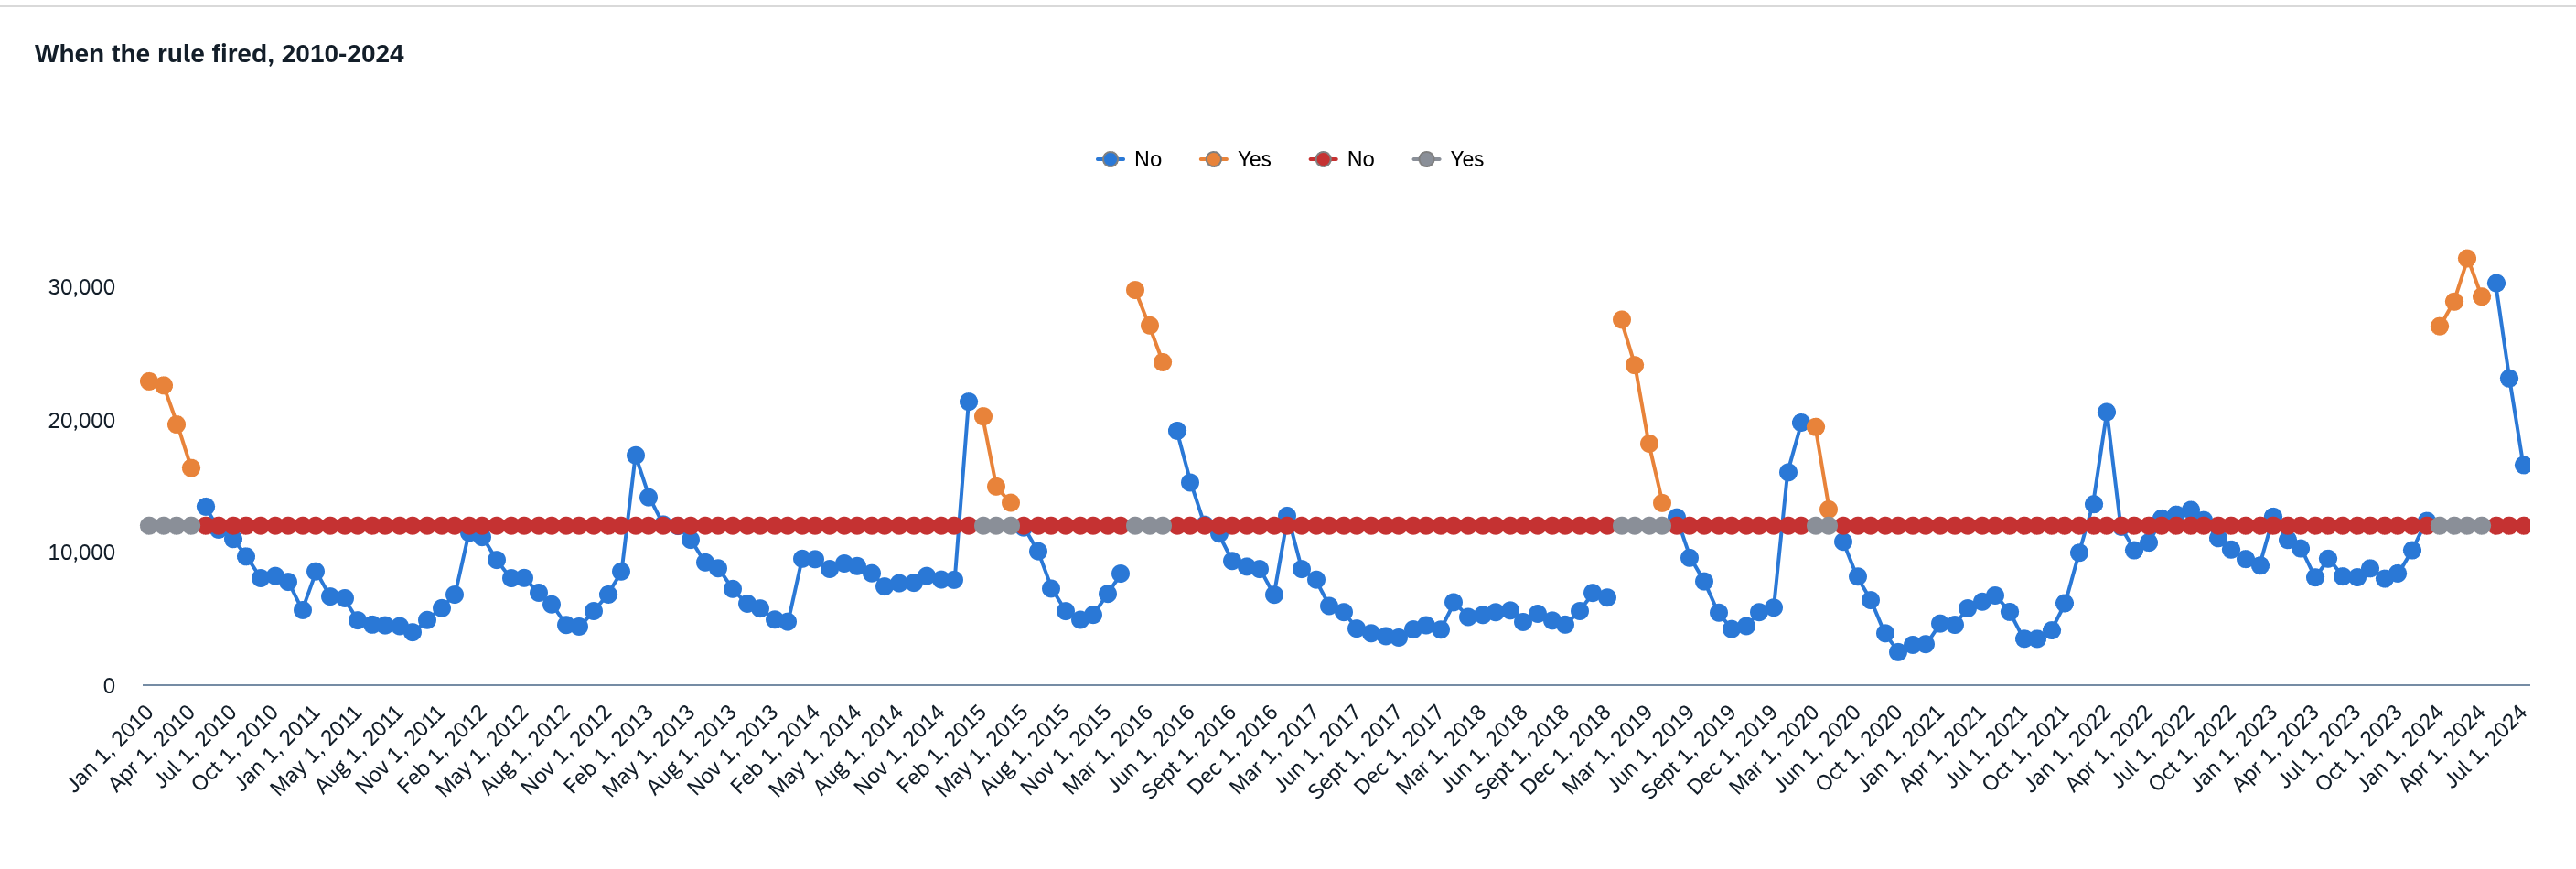
\includegraphics[width=420bp]{gambar-sac/h11-deret-aturan}};
  }{%
    \draw[rounded corners=3bp, fill=soft, draw=line, dashed] (48,214) rectangle ++(420,-142);
  }

  % ---- tabel pemangku kepentingan (sub-kriteria Viability: peran yang jelas)
  \node[anchor=north west, text=ink, font=\smlfont\bfseries] at (516,308)
    {Who does what};

  \node[anchor=north west] at (516,288) {%
    \begin{minipage}{408bp}
      \smlfont
      \setlength{\arrayrulewidth}{0.5bp}
      \arrayrulecolor{line}
      \renewcommand{\arraystretch}{1.34}
      \begin{tabular}{@{}>{\raggedright\arraybackslash}p{104bp}@{\hspace{12bp}}>{\raggedright\arraybackslash}p{292bp}@{}}
        \thd{Who} & \thd{Role}\\[-2bp]
        \hline
        \textbf{District health office} \textcolor{muted}{gov't}
          & Reads the advisory; moves PSN/3M, larviciding and stockpiles
            \emph{forward} into the alerted window\\
        \textbf{Ministry of Health $\cdot$ BMKG} \textcolor{muted}{gov't}
          & Own the monthly refresh; BMKG's forecast ONI stretches the notice
            past four months\\
        \textbf{\emph{Jumantik} cadres} \textcolor{muted}{NGO \& community}
          & Larval checks and household messaging concentrated in the alerted
            months instead of spread thin all year\\
        \textbf{Cloud \& telco partners} \textcolor{muted}{private}
          & Host the SAC tenant and the broadcast; one analyst-hour a month,
            no data team\\
        \hline
      \end{tabular}
    \end{minipage}};

  \draw[rounded corners=4bp, fill=soft, draw=none] (516,122) rectangle ++(408,-58);
  \node[anchor=north west, text=alarm, font=\eyefont] at (532,108) {SCALES BY SWAPPING ONE INPUT};
  \teks{532}{90}{376}{\tnyfont
    Thailand already validates with its own predictor (temperature anomaly,
    lag 2, lift 2.7). Any ASEAN member repeats the fit on its own records.}

  \kaki{The rule is the engine, not a feature of the product. Strip the dashboard
        away and a health office can still run \Produk{} on paper.}{15}
\end{halaman}

% =====================================================================
% REFERENSI — DI LUAR HITUNGAN 15 HALAMAN (aturan resmi panitia)
% Seluruh DOI diverifikasi lewat Crossref (judul + penulis + tahun + jurnal
% dicocokkan satu per satu), bukan disalin dari ingatan.
% =====================================================================
% REFERENSI — DI LUAR HITUNGAN 15 HALAMAN (aturan resmi panitia, boleh >1 hal.)
% Seluruh DOI diverifikasi lewat Crossref (judul + penulis + tahun + jurnal
% dicocokkan satu per satu), bukan disalin dari ingatan.
% =====================================================================
\newcommand{\rujuk}[1]{\par\vspace{4bp}#1}

\begin{halaman}
  \navbar{0}
  \kepala{References 1/2}{Data sources}

  \node[anchor=north west, text=alarm, font=\eyefont] at (\ML,\CTOP) {DATA};
  \teks{\ML}{406}{424}{\tnyfont
    OpenDengue V1.3. doi:10.6084/m9.figshare.24259573.v4
    \rujuk{World Bank Climate Change Knowledge Portal (ERA5 0.25\textdegree{}
      monthly temperature and precipitation).}
    \rujuk{NOAA Climate Prediction Center. Oceanic Ni\~no Index (ONI v5).}
    \rujuk{WHO/UNICEF Joint Monitoring Programme for Water Supply, Sanitation
      and Hygiene, 2025 update.}
    \rujuk{BPS-Statistics Indonesia. Provincial population, WebAPI.}
    \rujuk{European Commission JRC. Global Human Settlement Layer
      (GHS-UCDB R2019A).}
    \rujuk{SIPSN, Ministry of Environment and Forestry, Indonesia.}
    \rujuk{BNPB. Indonesian Disaster Data and Information (DIBI).}}

  \node[anchor=north west, text=alarm, font=\eyefont] at (\ML,236) {METHOD REFERENCE};
  \teks{\ML}{218}{424}{\tnyfont
    Hussain-Alkhateeb L, et al.\ (2017). \emph{Early warning and response system
    (EWARS) for dengue outbreaks: operational guide.} WHO/TDR technical document
    --- no DOI assigned; the peer-reviewed description is Hussain-Alkhateeb 2018
    on the next page.}

  \node[anchor=north west, text=alarm, font=\eyefont] at (500,\CTOP) {CLIMATE AND DENGUE};
  \teks{500}{406}{424}{\tnyfont
    Tian Y, et al.\ (2025). Rising dengue risk with increasing El
    Ni\~no--Southern Oscillation amplitude and teleconnections.
    \emph{Nat Commun}. doi:10.1038/s41467-025-63655-0
    \rujuk{Djaafara B, et al.\ (2026). Dengue transmission heterogeneity across
      Indonesia's archipelago: climate-driven spatiotemporal patterns and policy
      implications. \emph{PLOS Negl Trop Dis}. doi:10.1371/journal.pntd.0014135}
    \rujuk{Mokhtar S, et al.\ (2024). Global risk of dengue outbreaks and the
      impact of El Ni\~no events. \emph{Environ Res}.
      doi:10.1016/j.envres.2024.119830}
    \rujuk{Sutriyawan A, et al.\ (2025). Impact of climate change on dengue
      incidence: a systematic review of evidence from Southeast Asia.
      \emph{J Popul Soc Stud}. doi:10.25133/jpssv342026.028}
    \rujuk{Lowe R, et al.\ (2021). Combined effects of hydrometeorological
      hazards and urbanisation on dengue risk in Brazil.
      \emph{Lancet Planet Health}. doi:10.1016/S2542-5196(20)30292-8}
    \rujuk{Gibb R, et al.\ (2023). Interactions between climate change, urban
      infrastructure and mobility are driving dengue emergence in Vietnam.
      \emph{Nat Commun}. doi:10.1038/s41467-023-43954-0}
    \rujuk{Wang Y, et al.\ (2022). Impact of extreme weather on dengue fever
      infection in four Asian countries. \emph{Environ Int}.
      doi:10.1016/j.envint.2022.107518}
    \rujuk{Choi Y, et al.\ (2016). Effects of weather factors on dengue fever
      incidence and implications for interventions in Cambodia.
      \emph{BMC Public Health}. doi:10.1186/s12889-016-2923-2}
    \rujuk{Polrob P, et al.\ (2025). Nonlinear and lagged effects of climate
      variability on dengue incidence in Bangkok. \emph{BMC Public Health}.
      doi:10.1186/s12889-025-25420-2}}

  \kaki{Reference pages --- excluded from the 15-page limit per the official
        storyboard requirements. Every DOI was resolved against Crossref.}{R1}
\end{halaman}

\begin{halaman}
  \navbar{0}
  \kepala{References 2/2}{Early-warning systems, cost, and validation}

  \node[anchor=north west, text=alarm, font=\eyefont] at (\ML,\CTOP)
    {EARLY-WARNING SYSTEMS};
  \teks{\ML}{406}{424}{\tnyfont
    Hussain-Alkhateeb L, et al.\ (2018). Early warning and response system
    (EWARS) for dengue outbreaks: recent advancements towards widespread
    applications in critical settings. \emph{PLOS ONE}.
    doi:10.1371/journal.pone.0196811
    \rujuk{Baharom M, et al.\ (2022). Dengue early warning system as outbreak
      prediction tool: a systematic review. \emph{Risk Manag Healthc Policy}.
      doi:10.2147/RMHP.S361106}
    \rujuk{Benitez-Valladares D, et al.\ (2021). Validation of the early warning
      and response system (EWARS) for dengue outbreaks: evidence from the
      national vector control program in Mexico. \emph{PLOS Negl Trop Dis}.
      doi:10.1371/journal.pntd.0009261}
    \rujuk{C\'ardenas R, et al.\ (2022). The early warning and response system
      (EWARS-TDR) for dengue outbreaks: can it also be applied to chikungunya
      and Zika outbreak warning? \emph{BMC Infect Dis}.
      doi:10.1186/s12879-022-07197-6}
    \rujuk{Schlesinger P, et al.\ (2024). Enabling countries to manage outbreaks:
      statistical, operational, and contextual analysis of the EWARS-csd for
      dengue outbreaks. \emph{Front Public Health}. doi:10.3389/fpubh.2024.1323618}
    \rujuk{Quan TM, et al.\ (2026). Climatic determinants and simple thresholds
      for dengue early warning in Vietnam: a One Health perspective.
      \emph{Sci One Health}. doi:10.1016/j.soh.2026.100159}}

  \node[anchor=north west, text=alarm, font=\eyefont] at (500,\CTOP)
    {BURDEN, COST, AND VALIDATION};
  \teks{500}{406}{424}{\tnyfont
    Nadjib M, et al.\ (2019). Economic burden of dengue in Indonesia.
    \emph{PLOS Negl Trop Dis}. doi:10.1371/journal.pntd.0007038
    \rujuk{Wilastonegoro NN, et al.\ (2020). Cost of dengue illness in Indonesia
      across hospital, ambulatory, and not medically attended settings.
      \emph{Am J Trop Med Hyg}. doi:10.4269/ajtmh.19-0855}
    \rujuk{Shepard DS, et al.\ (2013). Economic and disease burden of dengue in
      Southeast Asia. \emph{PLOS Negl Trop Dis}. doi:10.1371/journal.pntd.0002055}
    \rujuk{Shepard DS, et al.\ (2016). The global economic burden of dengue: a
      systematic analysis. \emph{Lancet Infect Dis}.
      doi:10.1016/S1473-3099(16)00146-8}
    \rujuk{Sasmono RT, et al.\ (2026). Understanding the epidemiological trends
      and economic impact of dengue in Indonesia. \emph{IJID Regions}.
      doi:10.1016/j.ijregi.2026.100860}
    \rujuk{Childs ML, et al.\ (2025). Climate warming is expanding dengue burden
      in the Americas and Asia. \emph{PNAS}. doi:10.1073/pnas.2512350122}}

  \kaki{Reference pages --- excluded from the 15-page limit per the official
        storyboard requirements. Every DOI was resolved against Crossref.}{R2}
\end{halaman}

\end{document}
